% Source: fixed 2006 Zhejiang science scan, PDF page 1, Q17.
% Schematic oblique projection; labels and solid/hidden edge relations follow
% the printed figure. M and N lie on PC and PB respectively.
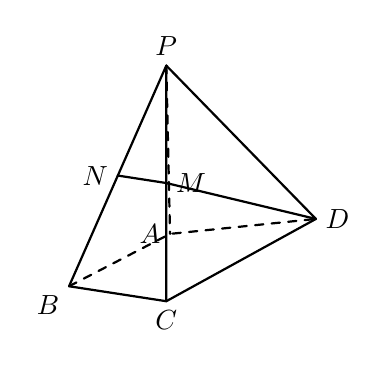
\begin{tikzpicture}[line cap=round,line join=round,x=0.95cm,y=0.95cm]
  \coordinate (P) at (1.55,3.1);
  \coordinate (A) at (1.6,0.85);
  \coordinate (B) at (0.25,0.15);
  \coordinate (C) at (1.55,-0.05);
  \coordinate (D) at (3.55,1.05);
  \coordinate (N) at (0.9,1.63);
  \coordinate (M) at (1.55,1.53);
  \draw[thick] (P)--(B)--(C)--(D)--cycle;
  \draw[thick] (P)--(C) (N)--(M)--(D);
  \draw[thick,dashed] (P)--(A) (B)--(A)--(D);
  \node[above] at (P) {$P$};
  \node[left] at (A) {$A$};
  \node[below left] at (B) {$B$};
  \node[below] at (C) {$C$};
  \node[right] at (D) {$D$};
  \node[left] at (N) {$N$};
  \node[right] at (M) {$M$};
\end{tikzpicture}
